\label{sec:foregrounds}

Cross-correlation of reionization-era 21\,cm observations with \lya\ intensity
mapping surveys have the advantage that 21\,cm foregrounds have no correlation with
the low redshift interloper lines that affect high-redshift \lya\ measurements.
Because the two are uncorrelated, power from the each of these foregrounds is not directly
added to the cross-power spectrum. However, while bright foregrounds do not contribute
to the amplitude on cross-power spectrum, they do contribute to the total variance
on the cross-power spectrum and must be accounted for.

For SPHEREx, the strategy of dealing with foregrounds for EoR measurements is simple:
remove voxels whose emission falls above some threshold value ($\sim 1.4 \times 10^{-20} \ \rm W / m^2$).
Estimates vary on the percentage of pixels that will to be masked to cut out near-infrared foregrounds.
For now, I assume that the spatial and spectral resolution is SPHEREx is fine enough
such that a small percentage of pixels are masked and that the amplitude of the
\lya\ power spectrum is not significantly changed as a result. Past
work estimates that for a SPHEREx-like experiment, roughly 3\% of pixels will need
to be masked to completely remove foregrounds (\cite{2014ApJ...785...72G}), so it seems like this might be reasonable
to assume for now. This may end up being a poor assumption to make and will likely require
further investigation to confirm. In the future, I will adopt a method of incorporating
pixel masking, such as randomly removing roughly 3\% of pixels, to identify its effect on the
cross-power spectrum spectrum detectability.

For HERA, there are two main strategies to deal with the foregrounds:
relying on the fact that the foregrounds are spectrally smooth, and thus confined
to an area of the 2D power spectrum known as the foreground wedge, and by precisely modeling
foregrounds and subtracting them from the data. There has been some success in subtracting
foregrounds from data in other 21\,cm experiments, such as with the Murchison Widefield Array (\cite{2019ApJ...884....1B}),
but because of the difficulty involved with modeling an instrument's response to foregrounds,
the primary foreground strategy for HERA will be the removal of the foreground wedge.

\begin{figure}[ht]
	\centering
	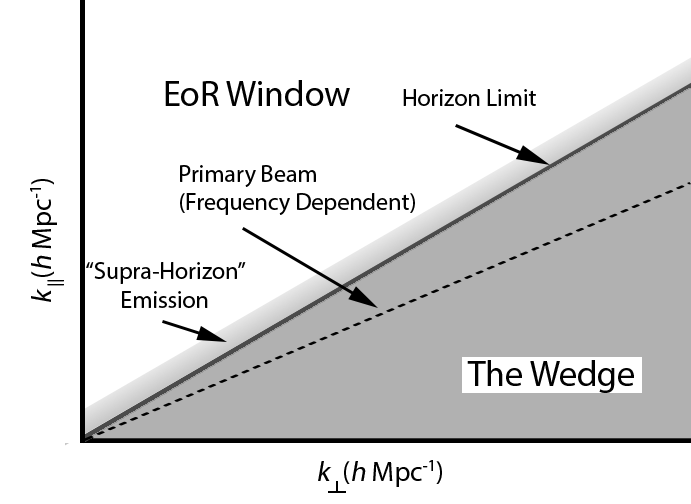
\includegraphics[width=0.9\textwidth]{wedge-diagram.png}
	\caption[Foreground Wedge]{A depiction of the cylindrically averaged 21\,cm power spectrum divided into
					the EoR window and the Wedge. Power from spectrally smooth foregrounds dominate the cosmological
					21\,cm signal at low $k_{\parallel}$ values and bleed into higher $k_{\parallel}$ modes the further
					they are from the field center, extending all the way to the horizon in cases of zenith-pointing
					telescopes such as HERA.}
	\label{fig:wedge}
\end{figure}

The foreground wedge is a well-documented feature in 21\,cm literature (\cite{2010ApJ...724..526D}, \cite{2012ApJ...752..137M})
and has been identified as a potential method of removing bright 21\,cm foregrounds.
To describe it simplistically, that 21\,cm foreground wedge is a feature that appears
in the cylindrically-averaged 21\,cm power spectrum that arises as a result of
spectral smooth foregrounds interacting with the chromatic response of an interferometer.
Because of their smooth spectral structure, bright foregrounds are defined by lower-order
Fourier modes, thus constraining their power to lower $k_{\parallel}$ values.
Power from more spectrally complex 21\,cm EoR signal requires higher-order Fourier modes to capture
its behavior and is pushed to a region of the 2D power spectrum known as the EoR window as a result.
Experiments, such as HERA, have leveraged the fact that the edge of the foreground wedge is dependent
on the baseline length of two antennas by building densely packed arrays that sample
lower $k_{\perp}$ values, thus increasing the EoR window. The exact relationship
defining the $k_{\parallel}$ edge of the wedge can be written as,
\begin{equation}
    k_{\parallel, \textrm{max}} \approx \theta_{0} k_{\perp} \frac{D_{M} \left( z \right) }{D_H} \frac{E \left( z \right)}{\left(1 + z\right)},
\end{equation}
where $\theta_{0}$ is the angle between the pointing center and bright foregrounds, $k_{\perp}$ is the Fourier mode
dependent on the distance between two dishes, and $k_{\parallel, \textrm{max}}$ corresponds to the
to the maximum $k_{\parallel}$ value dominated by bright foregrounds.
Typically, the safest assumption to make is that $\theta_{0} = \pi / 2$ which cooresponds
to bright foregrounds at the horizon, far from the pointing center. In practice,
the wedge can extend even beyond the horizon given improperly calibrated chromaticity
and mode-mixing effects. Fortunately, there have been results that show contamination
from the foregrounds have the potential to be contained within the field of view
of the instrument given precise calibration (\cite{2014ApJ...782...66P}).

To investigate the effect of the foreground wedge on the ability to measure the cross-power spectrum,
I adopt two treatments of 21\,cm foregrounds described in \cite{2014ApJ...782...66P}: a moderate foreground treatment,
where the foreground wedge extends to the horizon with a horizon buffer added, and an optimistic foreground treatment, where the wedge
is confined to the first null in the primary beam of the instrument. In both of these treatments,
I remove all samples that fall within the foreground wedge. The effect of the
wedge on the 21\,cm power spectrum can be observed in Figure \ref{fig:21cm_errors}.
For the moderate case, a large number of samples are removed from the data resulting
in the thermal noise dominating small $k$ values, while in the optimistic case,
many more of those modes are recovered and information on large-scale structure is
retained.

\begin{figure}[th]
	\centering
	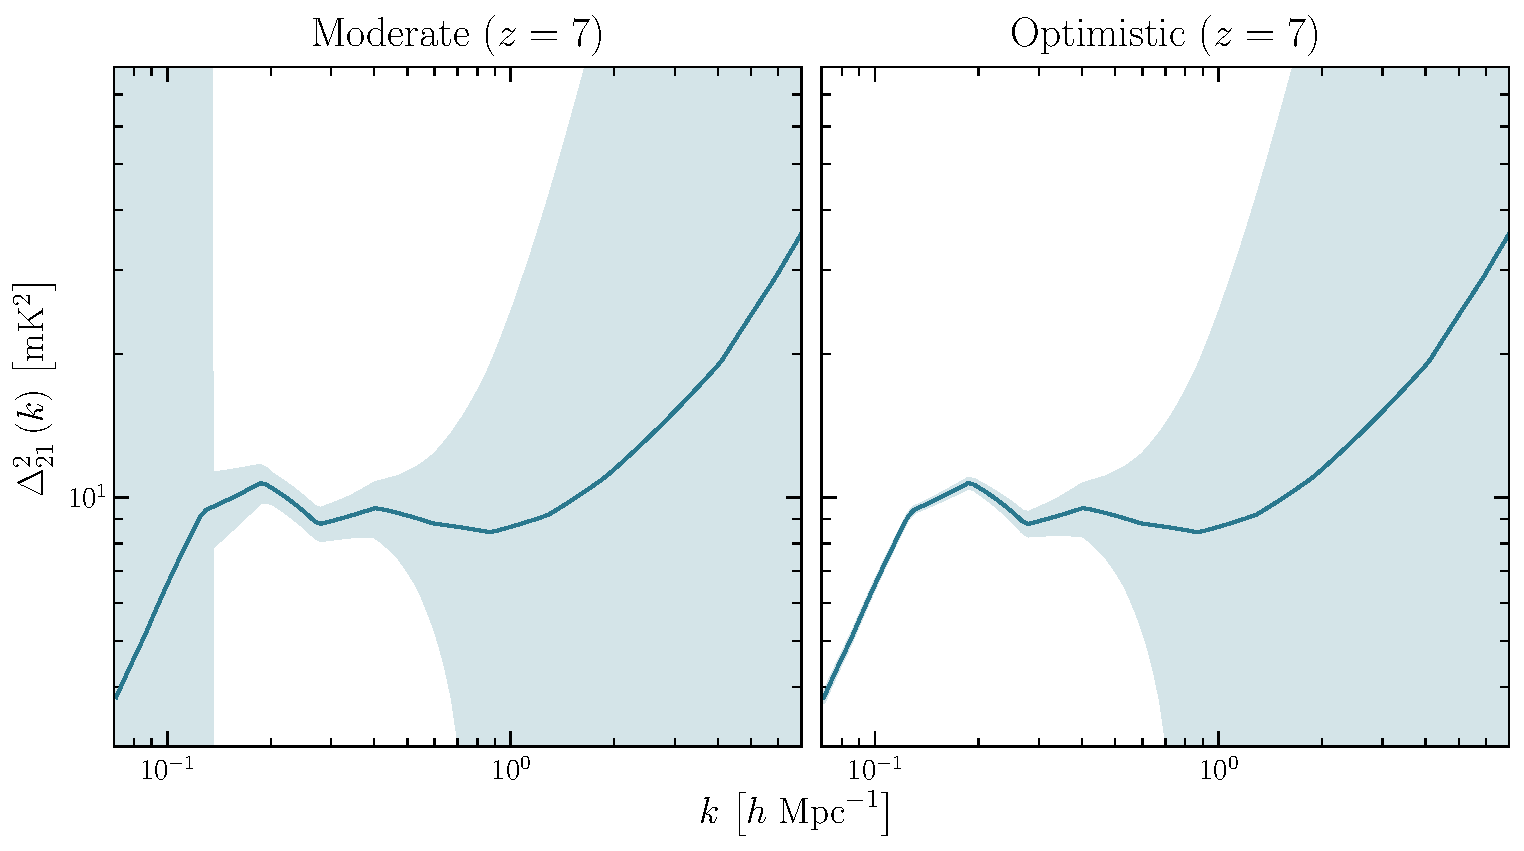
\includegraphics[width=1.0\textwidth]{21cm_errorbars.pdf}
	\caption[Optimistic vs. Moderate Foreground Treatment]{The 21\,cm power spectrum plotted with 1$\sigma$ errors given
																												 observing parameters stated in Table \ref{tab:obs_table}. Here, I compare the
																												 dependence of the two foreground cases on the noise. For the moderate case,
																												 all k-modes within the horizon limit are removed resulting in a complete loss of information on large scales $k \lesssim 0.15 \ h\,\textrm{Mpc}^{-1}$. For the optimistic case, foregrounds are confined to the first null in HERA's beam resulting in a much higher recovery of large scale information.}
	\label{fig:21cm_errors}
\end{figure}

\begin{figure}[th]
	\centering
	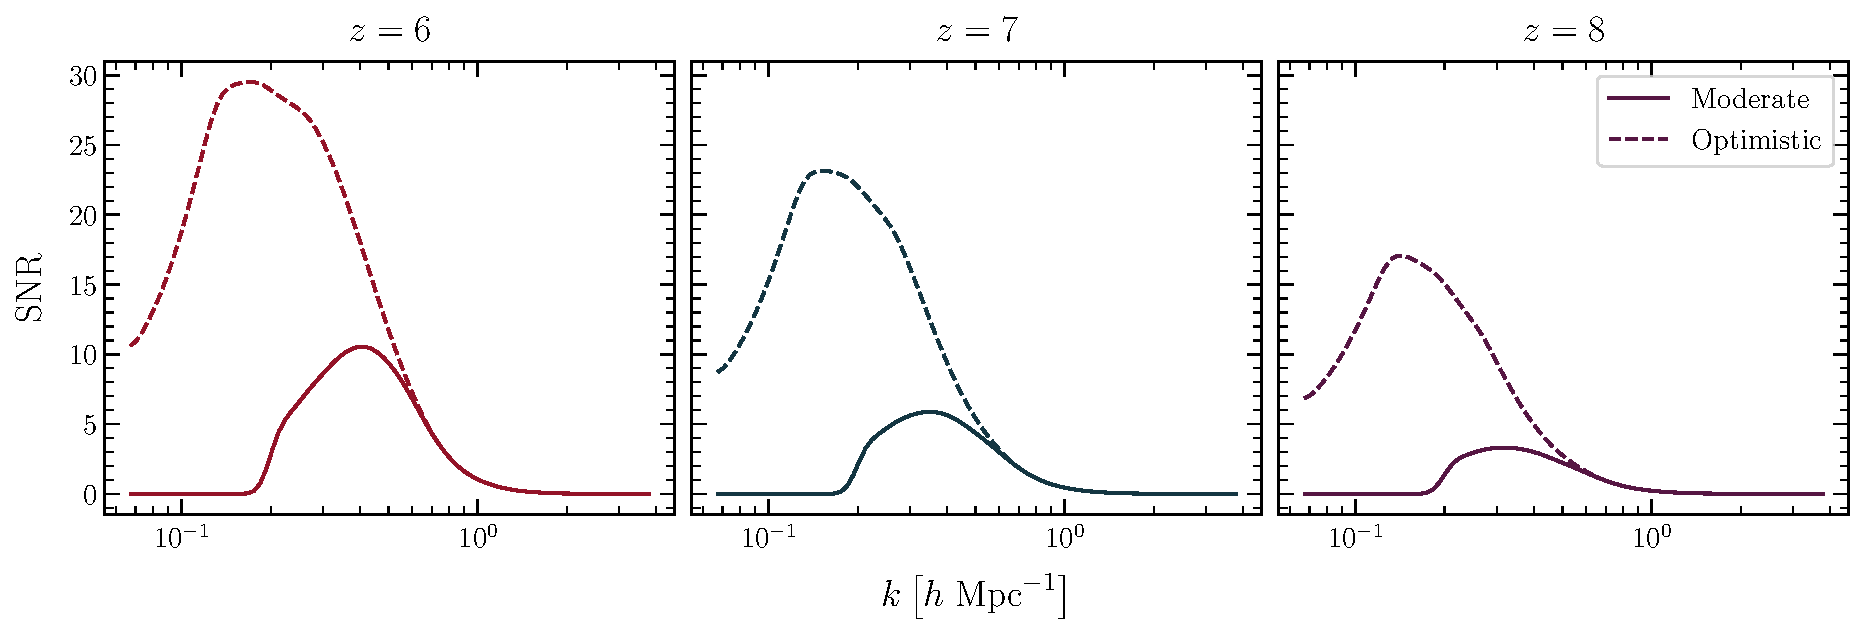
\includegraphics[width=0.95\textwidth]{xcorr_snr.pdf}
	\caption[Cross-Power Spectrum Signal-to-Noise]{Signal to noise estimates for the 21\,cm-\lya\ cross-power spectrum.
	The redshifts $z = [6, 7, 8]$ are plotted for both the optimistic and moderate foreground treatments. These estimates take
	into account the 21\,cm foreground wedge, thermal and sample variance from HERA and SPHEREx, and \lya\ attentuation due to
	absorption in the neutral IGM.}
	\label{fig:snr}
\end{figure}


Propagating these treatments of the 21\,cm foregrounds through to the cross-power spectrum, I arrive
at the final estimates on the sensitivity of the 21\,cm-\lya\ cross-power spectrum as measured
by HERA and SPHEREx while including thermal noise variance, sample variance, \lya\ attenuation,
and two treatments of the foreground wedge, shown in Figure \ref{fig:snr}. While it appears unlikely that a HERA-SPHEREx
cross-correlation measurement will be able to measure the cross-power spectrum turn-over,
it does appear to be able to make a high sensitivity measurement at large scales,
given an optimistic treatment of the foregrounds, and will even be able to make a detection
of the cross-power spectrum, assuming a moderate treatment of the foregrounds.

This result gives some confidence in the potential for HERA-SPHEREx synergies
in the future. Given even relatively conservative estimates, it seems that these
two instruments should be able to make a measurement of the cross-power spectrum
over their shared redshift range. While past work has shown that the 21\,cm-\lya\
cross-power spectrum should be a powerful probe of the EoR, it has yet to be seen
what information can be extracted from such a measurement with HERA and SPHEREx.
The next steps of this work will be to attempt to estimate reionization-era
parameters that seem to affect its progression the most through an MCMC analysis.
This should give some sense of how useful this metric will be at estimating the
underlying physics of reionization.
